\documentclass{article}
\usepackage[a4paper,margin=1.3cm]{geometry}
\usepackage{amsmath,amssymb,setspace,longtable,multirow,tikz,pgfplots,array,xcolor}
\usepackage{minted}
\usepackage[utf8]{inputenc}
\usepackage[T2A]{fontenc}
\usepackage[english,russian]{babel}
\usepackage{graphicx}
\setlength{\parindent}{2em}
\newcommand{\row}{\therow\addtocounter{row}{1}}
\newcounter{row}
\setcounter{row}{1}
\pgfplotsset{compat=1.16}
\newcolumntype{L}{>{\centering\arraybackslash}m{3cm}}
\definecolor{bg}{rgb}{0.96,0.96,0.93}
\setminted{frame=lines,framesep=1em}

\begin{document}
\begin{center}
    Национальный исследовательский университет ИТМО\\
    Факультет информационных технологий и программирования\\
    Прикладная математика
\end{center}
\vspace{20em}
\begin{center}
    {\Large — Линейное программирования}
    \vspace{3pt}
    \hrule
    \vspace{3pt}
    Отчет по лабораторной работе №1
\end{center}
\vspace{20em}
\begin{flushright}
    \textbf{ Работу выполнили: } \\
    Обиджанов Алишер\\
    Какзаков Андрей\\
    Кузнецов Павел\\
    \vspace{1em}
    \textbf{ Преподаватель: } \\
    Свинцов М.В.
\end{flushright}
\vspace{12em}
\begin{center}
    Санкт-Петербург \\
    2023
\end{center}
\newpage

\section{Теория}
Задача линейного программирования - максимизировать или минимизировать некоторый линейный функционал на многомерном пространстве при заданных линейных ограничениях.

Каждое из линейных неравенств на переменные ограничивает полупространство в соответствующем линейном пространстве. В результате все неравенства ограничивают некоторый выпуклый многогранник (возможно, бесконечный), называемый также полиэдральным комплексом.

Максимум функционала можно искать в вершинах многогранника. Принцип симплекс-метода состоит в том, что выбирается одна из вершин многогранника, после чего начинается движение по его рёбрам от вершины к вершине в сторону увеличения значения функционала. Когда переход по ребру из текущей вершины в другую вершину с более высоким значением функционала невозможен, считается, что оптимальное значение c найдено.

Последовательность вычислений симплекс-методом можно разделить на две основные фазы:

\begin{enumerate}
    \item Нахождение исходной вершины множества допустимых решений,
    \item Последовательный переход от одной вершины к другой, ведущей к оптимизации значения целевой функции.
\end{enumerate}

\section{Постановка задачи}
\begin{enumerate}
    \item Реализуйте возможность ввода данных из файла в формате JSON. Рекоменду-
          емая структура JSON указана ниже.
    \item При необходимости добавьте балансирующие переменные для перехода от об-
          щей постановки к канонической форме задачи линейного программирования.
    \item Реализуйте симплекс-метод для решения задачи.
    \item Предусмотрите, что задача как может не иметь решений вообще, так и иметь
          бесконечное количество решений
\end{enumerate}

\section{Реализация}

\subsection{Подключаем библиотеки}

\begin{listing}[H]
    \begin{minted}{python}
    import numpy as np
    from json import loads
    \end{minted}
\end{listing}

\subsection{Подготавливаем пример в формате json}
\begin{listing}[H]
    \begin{minted}{python}
    example = """{"f": [1, 2, 3],
              "goal": "max",
              "constraints": [{"coefs": [1, 0, 0],
                                "type": "eq",
                                "b": 1},
                               {"coefs": [1, 1, 0],
                                "type": "gte",
                                "b": 2},
                               {"coefs": [1, 1, 1],
                                "type": "lte",
                                "b": 3}]}"""
    \end{minted}
\end{listing}

\subsection{Парсим json файл}

Преобразует json в матрицы f, A и b, которые затем возвращает. Если задача имеет цель "min", то целевая функция домножается на -1.
Коэффициенты у всех ограничений в виде неравенств вида "больше" инвертируются, тем самым превращаясь в ограничния вида "меньше".
Когда встречается равенство, оно делится на два неравенства, одно с неизменённым знаком, другое - с изменённым.

\begin{listing}[H]
    \begin{minted}{python}
def parse_problem(json: str):
    parsed = loads(json)
    f = np.array(parsed['f'])
    A = []
    b = []
    for constraint in parsed['constraints']:
        A.append(np.array(constraint['coefs']))
        b.append(constraint['b'])
        if constraint['type'] == "gte":
            A[-1] *= -1
            b[-1] *= -1
        if constraint['type'] == "eq":
            A.append(np.array(constraint['coefs']) * -1)
            b.append(-constraint['b'])
    A = np.array(A)
    A = np.hstack((A, np.eye(A.shape[0])))
    b = np.array(b)
    return f, A, b, parsed['goal'] == "min"
    \end{minted}
\end{listing}

\subsection{Симплекс-метод}

Сначала создается таблица tableau, которая объединяет матрицы A и b. Если в таблице есть отрицательные элементы в столбце b, то выбирается строка i с минимальным значением b и столбец l с минимальным значением в этой строке. Затем находятся отношения между элементами строки i и столбцом l и выбирается строка r с наименьшим отношением. Далее выполняется шаг симплекс-метода для выбранных строк и столбцов.

\subsubsection{Шаг симплекс-метода}
\begin{listing}[H]
    \begin{minted}{python}
    def simplex_step(tableau, r, l):
    print(f"doing smplex step with {r=} and {l=}")
    for i in range(tableau.shape[0]):
        if i == r:
            tableau[i] /= tableau[i, l]
            continue
        tableau[i] -= tableau[r] * tableau[i, l] / tableau[r, l]
    \end{minted}
\end{listing}

\subsubsection{Симплекс-метод}
\begin{listing}[H]
    \begin{minted}{python}
        def simplex(f, A, b: np.ndarray, isMin):
        tableau = np.hstack((b.reshape(-1, 1), A))
        tableau = np.vstack((tableau, np.hstack((np.zeros((1,)), f, np.zeros((A.shape[0]))))))
        print(tableau)
        basis = np.arange(A.shape[0], A.shape[0] * 2) - 1
        print(basis)
        while (tableau[:-1, 0].min() < 0):
            i = tableau[:-1, 0].argmin()
            l = tableau[i, 1:].argmin() + 1
            if tableau[i, l] >= 0:
                raise Exception("No solution.")
            ratios = tableau[:-1, 0] / tableau[:-1, l]
            r = np.where(ratios > 0, ratios, np.inf).argmin()
            simplex_step(tableau, r, l)
            basis[r] = l
            print(tableau)
        s = (tableau[-1, 1:].argmax() if isMin else tableau[-1, 1:].argmin()) + 1
        last_max = -1
        while tableau[-1, 1:].min() < 0 if isMin else tableau[-1, 1:].max() > 0:
            # print(tableau[:-1, s])
            temp = tableau[:-1, s]
            temp[temp == 0] = -1
            ratios = tableau[:-1, 0] / temp
            print(f"ratios:\n{ratios}")
            j = ratios.argmin()
            simplex_step(tableau, j, s)
            basis[j] = s
            print(basis)
            print(tableau)
            s = (tableau[-1, 1:].argmax() if isMin else tableau[-1, 1:].argmin()) + 1
            if tableau[-1, s] == last_max:
                break
            last_max = tableau[-1, s]
        return -tableau[-1, 0]

    \end{minted}
\end{listing}

\section{Результат}
\begin{listing}[H]
    \begin{minted}{python}
    print(simplex(*parse_problem(example)))
    \end{minted}
\end{listing}

\textbf{Output:}

$$\begin{pmatrix}
        1 & 1  & 0  & 0 & 1  & 0 & 0 & 0 \\
        0 & 0  & 0  & 0 & 1  & 1 & 0 & 0 \\
        0 & 1  & -1 & 0 & 2  & 0 & 1 & 0 \\
        0 & -2 & 1  & 1 & -3 & 0 & 0 & 1 \\
        0 & 1  & 2  & 3 & 0  & 0 & 0 & 0
    \end{pmatrix}$$

$$\begin{pmatrix}
        0 & 0 & 0 & 1
    \end{pmatrix}$$

$$\begin{pmatrix}
        -1 & -1 & -0 & 1 & -1 & -0 & -0 & -0 \\
        -1 & -1 & 0  & 0 & 0  & 1  & 0  & 0  \\
        -1 & 0  & -1 & 0 & 1  & 0  & 1  & 0  \\
        1  & -1 & 1  & 0 & -2 & 0  & 0  & 1  \\
        3  & 4  & 2  & 0 & 3  & 0  & 0  & 0
    \end{pmatrix}$$

$$\begin{pmatrix}
        -1 & -1 & 0 & -1
    \end{pmatrix}
$$

$$\begin{pmatrix}
        -2 & 0 & -1 & 1  & 1  & -0 & -0 & -1 \\
        -2 & 0 & -1 & 0  & 2  & 1  & 0  & -1 \\
        -2 & 0 & -2 & 0  & 3  & 0  & 1  & -1 \\
        -1 & 1 & -1 & -0 & 2  & -0 & -0 & -1 \\
        7  & 0 & 6  & 0  & -5 & 0  & 0  & 4
    \end{pmatrix}$$

$$7.0$$

\section{Тестирование}
\subsection{Задачи для тестирования}
\begin{listing}[H]
    \begin{minted}{json}
        [
            {"task": {
                "f": [1, 2, 3],
                "goal": "max",
                "constraints": [{"coefs": [1, 0, 0],
                                "type": "eq",
                                "b": 1},
                                {"coefs": [1, 1, 0],
                                "type": "gte",
                                "b": 2},
                                {"coefs": [1, 1, 1],
                                "type": "lte",
                                "b": 3}]},
            "correct_answer": 3.0
            },
            {
            "task":{
                "f":[3, 4],
                "goal": "max",
                "constraints":[{"coefs":[-1, 1],
                                "type":"lte",
                                "b":3},
                                {"coefs":[5, 3],
                                "type":"lte",
                                "b":97},
                                {"coefs":[1, 7],
                                "type":"gte",
                                "b":74}]},
                "correct_answer": 58.375
            },
            {
            "task":{
                "f":[5.2, -1],
                "goal": "min",
                "constraints":[{"coefs":[2, 5],
                                "type":"gte",
                                "b":10},
                                {"coefs":[1, -3],
                                "type":"lte",
                                "b":3},
                                {"coefs":[-1, 1],
                                "type":"lte",
                                "b":1}]},
                "correct_answer": 2
            },
            {
                "task":{
                "f":[-3, 1, 4, 0, 0],
                "goal": "max",
                "constraints":[{"coefs":[0, -1, 1, 1, 0],
                                "type":"eq",
                                "b":1},
                                {"coefs":[-5, 1, 1, 0, 0],
                                "type":"eq",
                                "b":2},
                                {"coefs":[-8, 1, 2, -1, 0],
                                "type":"eq",
                                "b":3}]},
                "correct_answer": 10
            }
        ]        
    \end{minted}
\end{listing}


\subsection{Результат тестов}

\begin{figure}[H]
    \centering
    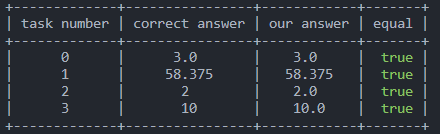
\includegraphics [width=1\textwidth]{2023-11-29-22-39-57.png}\\
    \caption{}
\end{figure}


\section{Вывод}

В ходе данной лабораторной работы был реализован симплекс-метод для решения задачи линейного программирования. Была предусмотрена возможность ввода данных из файла в формате JSON. Были добавлены балансирующие переменные для перехода от общей постановки к канонической форме задачи линейного программирования.
\end{document}
